\chapter{The finite element code Legolas} \label{ch: Legolas}

\graphicspath{{04-legolas/figures/}}

\usespublishedwork{
  Most of this Chapter was published in ``Legolas: a novel tool for magnetohydrodynamic spectroscopy'', 2020, \apjs,
  251, 25 \citep{claes2020_legolas}. N. Claes developed Legolas in close collaboration with J. De Jonghe, generated the data and figures and wrote a first draft of the manuscript; J. De Jonghe revised and extended the manuscript. R. Keppens contributed to the revision of the paper.
}

\section{Introduction}

\section{Problem description and equations}
In this Section we will develop the mathematical formalism leading up to the set of linearised equations. The inhomogeneous equilibrium profiles under consideration make the linearisation process much more complicated compared to Chapter \ref{ch: spectroscopy}, and we also include a lot more physical effects than before.

\subsection{Full set of MHD equations}
We start from the same set of MHD equations as in Chapter \ref{ch: spectroscopy}, but now we include a gravitational field, resistivity, and background flow effects, in addition to optically thin radiative losses and anisotropic thermal conduction. This implies that the initial set of MHD equations expands into
\begin{flalign}
  \frac{\partial \rho}{\partial t} &= -\nabla \cdot (\rho \bv), \label{eq: continuity} \\
  \rho\frac{\partial \bv}{\partial t} &=
    -\nabla p - \rho \bv \cdot \nabla \bv + (\nabla \times \bb) \times \bb + \rho\bg
    + \mu\left[\nabla^2\bv + \frac{1}{3}\nabla(\nabla \cdot \bv)\right],	\label{eq: momentum} \\
  \rho\frac{\partial T}{\partial t} &=
    -\rho \bv\cdot\nabla T - \gmone p\nabla \cdot \bv - \gmone\rho\HLF
    + \gmone\nabla \cdot (\bkappa \cdot \nabla T) \label{eq: energy} \\
    &\quad + \gmone\eta(\nabla \times \bb)^2 + \mu\left|\nabla \bv \right|^2 \nonumber \\
  \frac{\partial \bb}{\partial t} &=
    \nabla \times (\bv \times \bb) - \nabla \times (\eta\nabla \times \bb) \label{eq: induction}
\end{flalign}
Here $\eta$ denotes the resistivity, $\bg$ the gravitational acceleration, and $\mu$ the dynamic viscosity assumed to be constant. It is worth noting that {\legolas} also includes a full Hall MHD treatment consisting of the regular Hall term, electron pressure term and electron inertia term, although this will not be discussed in the scope of this thesis.

\subsection{Linearisation of the physical terms}
\subsubsection{Equilibrium background}
Just as in Chapter \ref{ch: spectroscopy} we need a background around which to linearise. Since we want our mathematical formalism to be quite general, we consider a coordinate system denoted by $(u_1, u_2, u_3)$, corresponding to three orthogonal basis vectors. The main advantage of this approach is that it allows us to include two different geometries with only one basic formalism (and implementation). First we consider a standard plane slab geometry in Cartesian coordinates, that is, a plasma which is confined in height and considered to be bounded by two horizontal, perfectly conducting walls at a fixed distance apart, extending outwards to infinity in the other two ignorable coordinates. This also approximates the limit of a fully infinite free space when the walls are moved off to infinity. In Cartesian geometry the coordinate system can be written as $(x, y, z)$ and the vectors $\{\uunit{1}, \uunit{2}, \uunit{3}\}$ are then the standard Cartesian triad $\{\unit{x}, \unit{y}, \unit{z}\}$ along the axes. This makes it quite convenient to include for example gravitational effects which will induce an equilibrium stratification in the $u_1$ coordinate. The second geometry under consideration is that of an infinitely long plasma cylinder encased by a solid wall at a certain radius away from the cylinder axis, for which the coordinate system can be defined as $(r, \theta, z)$. At each point the vectors $\{\uunit{1}, \uunit{2}, \uunit{3}\}$ are defined as the triad of tangent vectors, $\{\unit{r}, \munit{\theta}, \unit{z}\}$, with $\unit{r}$ along the radial direction, $\unit{z}$ in the direction of the cylinder axis and $\munit{\theta} = \unit{z} \times \unit{r}$ tangent to the cylinder.
The basic operators present in Equations \eqref{eq: continuity}--\eqref{eq: induction}, that is, the divergence, gradient and curl, introduce a factor $r$ when going from Cartesian to cylindrical coordinate systems. To make life easy we can introduce the \emph{scale factor} $\eps = r$ for cylindrical geometries, which is reduced to $\eps = 1$ for a Cartesian coordinate system. Hence exploiting this scale factor in the mathematical formalism allows for one single implementation, where one can conveniently switch between both cases. We note that the cylindrical setup is also applicable to the so-called cylindrical accretion disk limit, as for example exploited to study MHD instabilities in disks by \citet{blokland2007}.

We again linearise the above set of MHD equations and similar to before this involves splitting variables into two parts: a time-independent part denoted with subscript 0, and a perturbed part denoted by a subscript 1. \legolas~ handles one-dimensional equilibria which depend only on $u_1$, or, more specifically, time-independent equilibria of the form
\begin{equation}	\label{eq: legolas_equilibrium}
	\begin{aligned}
		\rho_0 &= \rho_0(u_1),		\\
		p_0 &= p_0(u_1),			\\
		T_0 &= T_0(u_1),			\\
	\end{aligned}
	\qquad\qquad
	\begin{aligned}
		\bv_0 &= v_{01}(u_1)\uunit{1} + v_{02}(u_1)\uunit{2} + v_{03}(u_1)\uunit{3},	\\
		\bb_0 &= B_{01}\uunit{1} + B_{02}(u_1)\uunit{2} + B_{03}(u_1)\uunit{3}. \\
		&
	\end{aligned}
\end{equation}
In general we have $\bg = -g(u_1)\uunit{1}$, where the Cartesian case is for a stratified atmosphere or layer, and the cylindrical case can also allow for gravitational stratification of an accretion disk situated for $u_1 = r \in [1, R]$. In the case of a cylinder where $u_1 = r \in [0, R]$, this gravitational term is absent. The presence of a $u_1$-dependent $\uunit{1}$ component in the velocity field allows for compressible background flows, that is, $\nabla \cdot \bv_0 \neq 0$. It should be noted that in order for $\nabla \cdot \bb_0 = 0$ to hold, we actually need $B_{01}/\eps$ as $\uunit{1}$ component for the magnetic field, which reduces to the constant $B_{01}$ in Cartesian geometries and $B_{01}/r$ for cylinders. However, we will not consider the latter case as it will introduce even more terms in the equations, hence at the time of writing {\legolas} only allows for a non-zero $B_{01}$ component in Cartesian slabs.

\begin{figure}[t]
  \centering
  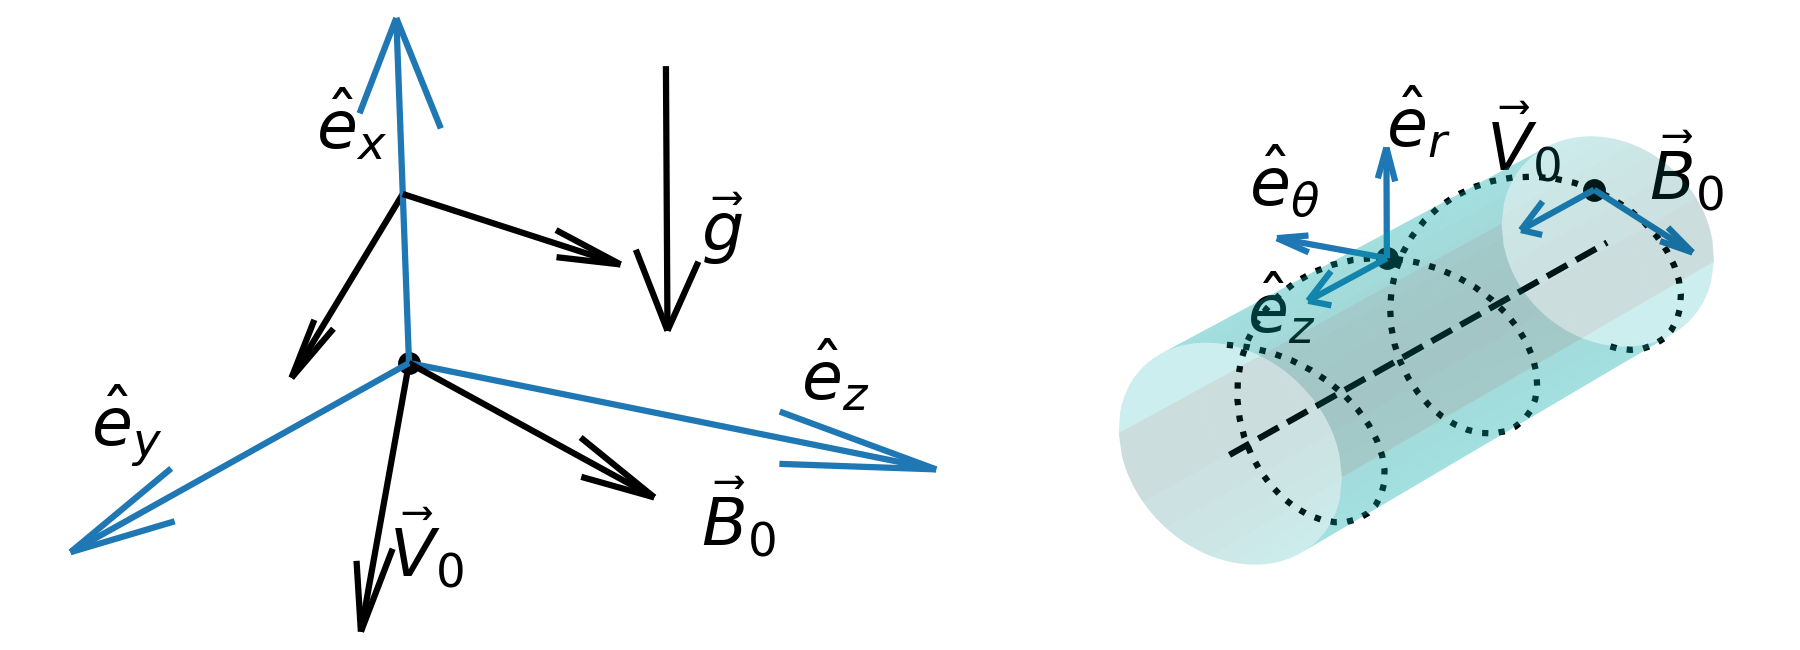
\includegraphics[width=\textwidth]{coordinate_axes.png}
  \caption{
    Unit vectors and examples of $\bb_0$ and $\bv_0$ for the Cartesian (\textbf{left}) and cylindrical (\textbf{right}) cases. These correspond to the general formalism given by Equation \eqref{eq: legolas_equilibrium}
    with $v_{01} = B_{01} = 0$.
  }
  \label{fig: coordinate_axes}
\end{figure}

In what follows the $v_{01}(u_1)$ and $B_{01}$ terms are included in the mathematical formalism for completeness, but will be set to zero in all applications discussed in the remainder of this thesis. Essentially, this implies that the general formalism in Equation \eqref{eq: legolas_equilibrium} reduces to the configuration shown on Figure \ref{fig: coordinate_axes}.

\subsubsection{Resistive terms}
The resistivity contribution in the energy equation is given by $\gmone \eta (\nabla \times \bb)^2$, which can be straightforwardly linearised as
\begin{equation}
  \begin{gathered}
    \gmone\left(\eta_0 + \eta_1\right)\left(\nabla \times \bb_0 + \nabla \times \bb_1\right)^2 \\
    = 2\gmone \eta_0 \left(\nabla \times \bb_0\right) \cdot \left(\nabla \times \bb_1\right)
      + \gmone\eta_1 \left(\nabla \times \bb_0\right) \cdot \left(\nabla \times \bb_0\right),
  \end{gathered}
\end{equation}
in which the nonlinear terms and equilibrium contributions were omitted. For the resistivity $\eta$ one can in principle take any profile, {\legolas} implements the Spitzer resistivity given by
\begin{equation} \label{eq: spitzer_eta}
  \eta = \frac{4\sqrt{2\pi}}{3}\frac{
    Z_\text{ion} \electroncharge^2 \sqrt{\masse} \ln(\lambda)
  }{
    \left(4\pi\epsilon_0\right)^2\left(\boltzmanncte T\right)^{3/2}
  },
\end{equation}
where $Z_\text{ion}$ denotes the ionisation taken to be unity, $\electroncharge$ and $\masse$ denote the electron charge and mass, respectively, and $\epsilon_0$ and $\boltzmanncte$ are the electrical permittivity and Boltzmann constant. The Coulomb logarithm is given by $\ln(\lambda)$ and is approximately equal to 22 for solar coronal conditions \citep{book_MHD}. It is important to emphasise that, since we will further linearise the governing nonlinear equations, we can adopt fully realistic values for all the nonideal coefficients, such as the resistivity or thermal conduction coefficients. This is in contrast to fully nonlinear computations, which are severely restrained in reaching magnetic Reynolds numbers $\magneticreynolds$ beyond $10^4$--$10^5$. The assumption of Spitzer resistivity implies that the perturbed part $\eta_1$ can be written in terms of perturbed temperature as
\begin{equation}
  \eta_1 = \left.\frac{d\eta}{dT}\right|_{T_0}T_1.
\end{equation}

\subsubsection{Optically thin radiative losses}
Just as before the optically thin radiative losses are governed by the heat-loss function $\HLF$, and the radiative cooling term $\gmone \rho \HLF$ in the energy equation can be linearised as
\begin{equation}
  \gmone \rho_1 \HLF_0 + \gmone \rho_0 \HLF_1.
\end{equation}
This time however we generalise the formalism to include a density and temperature-dependent heating function
$\HLFheat(\rho, T)$, such that the perturbed heat-loss function can be written as
\begin{equation} \label{eq: perturbed_HLF}
  \HLF_1 = \left(
    \Lambda(T_0) - \left.\frac{\partial \HLFheat(\rho, T)}{\partial \rho}\right|_{\rho_0, T_0}
  \right)\rho_1 + \left(
    \rho_0 \left.\frac{\partial \HLFcool}{\partial T}\right|_{T_0}
    - \left.\frac{\partial \HLFheat(\rho, T)}{\partial T}\right|_{\rho_0, T_0}
  \right) T_1,
\end{equation}
which can be set equivalent to $\HLF_1 = \dHLFrho\rho_1 + \dHLFT T_1$. {\legolas} has multiple cooling curves implemented, most notably {\jccorona} and {\spexdm} as shown on Figure \ref{fig: coolingcurves}. In addition a piecewise power law as described by \citet{rosner1978} is also implemented, which is an explicit (piecewise) function over the entire temperature domain.

\subsubsection{Anisotropic thermal conduction}
The thermal conduction term $\nabla \cdot (\bkappa \cdot \nabla T)$ in the energy equation is quite straightforward to linearise:
\begin{equation}
  \nabla \cdot \left(\bkappa_0 \cdot \nabla T_1\right) + \nabla \cdot \left(\bkappa_1 \cdot \nabla T_0\right).
\end{equation}
However, as we are dealing with a tensor quantity to model the anisotropy in MHD, the linearisation \emph{process} is tricky. Rewriting the tensor expression \eqref{eq: conduction} as
\begin{equation}
  \bkappa = \left(\kappapara - \kappaperp\right)\unit{B}\unit{B} + \kappaperp\idmat,
\end{equation}
where $\unit{B} = \bb/B_0$ is the unit vector along the magnetic field. So in addition to having to linearise the thermal conduction coefficients, we \emph{also} have to linearise this unit vector to account for a change in tensor directions. This implies that $\unit{B}\unit{B}$ is linearised as
\begin{equation} \label{eq: linearised_eB}
  \begin{gathered}
    \underbrace{
      \unit{B$_0$}\unit{B$_0$}
      + \unit{B$_1$}\unit{B$_0$}
      + \unit{B$_0$}\unit{B$_1$}
    }_\text{``regular'' terms}
    \underbrace{
      - \unit{B$_0$}\unit{B$_0$}\left(\unit{B$_0$} \cdot \unit{B$_1$}\right)
      - \unit{B$_0$}\unit{B$_0$}\left(\unit{B$_1$} \cdot \unit{B$_0$}\right)
    }_\text{change in tensor directions} \\
    = \unit{B$_0$}\unit{B$_0$} + \unit{B$_1$}\unit{B$_0$} + \unit{B$_0$}\unit{B$_1$}
      - 2\unit{B$_0$}\unit{B$_0$}\left(\unit{B$_0$} \cdot \unit{B$_1$}\right).
  \end{gathered}
\end{equation}
In what follows we can use the identity
\begin{equation} \label{eq: divergence_expression}
  \nabla \cdot (\bb_0 f) = f\nabla \cdot \bb + \bb_0 \cdot \nabla f,
\end{equation}
with $f$ a scalar term, the first term drops out since $\nabla \cdot \bb = 0$. Additionally, to shorten the notation we introduce the symbol
\begin{equation}
  \kappapfK{j} \equiv \frac{\skappapara{j} - \skappaperp{j}}{B_0^2},
\end{equation}
in which $j$ is either 0 or 1, denoting the unperturbed or perturbed parts, respectively.

\paragraph{Unperturbed tensor part} This part is given by $\nabla \cdot \left(\bkappa_0 \cdot \nabla T_1\right)$, which becomes
\begin{equation}
  \begin{gathered}
    \nabla \cdot \Bigl[(\skappapara{0} - \skappaperp{0})\unit{B$_0$}\unit{B$_0$} \cdot \nabla T_1\Bigr]
      + \nabla \cdot (\skappaperp{0}\nabla T_1) \\
    = \bb_0 \cdot \nabla \left(\kappapfK{0} \bb_0 \cdot \nabla T_1\right)
      + \nabla \cdot \left(\skappaperp{0}\nabla T_1\right).
  \end{gathered}
\end{equation}


\paragraph{Perturbed tensor part} This is given by $\nabla \cdot \left(\bkappa_1 \cdot \nabla T_0\right)$ and can be worked out in a similar way as the unperturbed part. Substituting a vector potential $\bb_1 = \nabla \times \ba_1$ and combining Equation \eqref{eq: linearised_eB} with \eqref{eq: divergence_expression} yields
\begin{equation}
  \begin{gathered}
    \bb_0 \cdot \nabla \left(\kappapfK{1}\bb_0 \cdot \nabla T_0\right)
    + \nabla \cdot \left(\skappaperp{1} \nabla T_0\right) \\
    + \left(\nabla \times \ba_1\right) \cdot \nabla \left(\kappapfK{0} \bb_0 \cdot \nabla T_0\right)
    + \bb_0 \cdot \nabla \Bigl(\kappapfK{0}\left(\nabla \times \ba_1\right) \cdot \nabla T_0\Bigr) \\
    - \bb_0 \cdot \nabla \left[
      2\kappapfK{0}\frac{1}{B_0^2}\bb_0 \Bigl(\bb_0 \cdot (\nabla \times \ba_1)\Bigr) \cdot \nabla T_0
    \right].
  \end{gathered}
\end{equation}
Note that the first, third and last terms drop out if we have no $B_{01}$ component, since in that case
$\bb_0 \cdot \nabla T_0 = 0$, which in turn implies that there is no $\skappapara{1}$ contribution.
This is no longer the case if a constant $B_{01}$ component would be present, then all these terms are nonzero.

\paragraph{Perturbed conduction coefficients} If we assume Spitzer conductivity as in Equation \eqref{eq: thermal_coeffs}, i.e. $\kappapara(T)$ and $\kappaperp(\rho, T, \bb)$, then we can write the perturbed thermal conduction coefficients in terms of the other variables:
\begin{equation}
  \skappapara{1} = \frac{\partial \kappapara}{\partial T} T_1,
\end{equation}
and
\begin{equation}
  \begin{aligned}
    \skappaperp{1} &=
      \frac{\partial \kappaperp}{\partial \rho}\rho_1
      + \frac{\kappaperp}{\partial T}T_1
      + \frac{\partial \kappaperp}{\partial B}\frac{\bb_0 \cdot \bb_1}{B} \\
    &= \frac{\partial \kappaperp}{\partial \rho}\rho_1
      + \frac{\kappaperp}{\partial T}T_1
      + 2\bb_0\cdot\bb_1 \frac{\partial \kappaperp}{\partial\left(B^2\right)},
  \end{aligned}
\end{equation}
where we used $\dfrac{\partial \kappaperp}{\partial (B^2)} = \dfrac{\partial \kappaperp}{\partial B}\dfrac{1}{2B}$.

\subsubsection{Viscosity}
The viscous force addition to the momentum equation is given in tensorial form by
$\mathbf{F}_{\mathrm{visc}} = -\nabla\cdot\left(\mu\mathbf{\Pi}\right)$, which for constant dynamic viscosity $\mu$ can be simplified to good approximation to
\begin{equation}
	\mathbf{F}_{\mathrm{visc}} \simeq \mu \left[ \nabla^2\bv + \frac{1}{3} \nabla\left(\nabla\cdot\bv\right)\right].
\end{equation}
This relies on splitting the tensor in a symmetric and antisymmetric part, as explained in \citet{porth2014_amrvac}. Linearising this yields
\begin{equation}
  \mu\left[\nabla^2\bv_1 + \frac{1}{3}\nabla(\nabla \cdot \bv_1)\right].
\end{equation}
In the energy equation we have a viscous heating term $\mu \left|\nabla \bv\right|^2$, where we assume that the norm here (which is essentially the norm of a matrix) represents the Frobenius norm such that
\begin{equation}
  \mu\left|\nabla \bv\right|^2 = \mu\sum_{i=1}^{3}\sum_{j=1}^{3}\left(\nabla \bv\right)_{ij}^2,
\end{equation}
which can be linearised as
\begin{equation}
  2\mu\sum_{i=1}^{3}\sum_{j=1}^{3}\left(\nabla \bv_0\right)_{ij}\left(\nabla \bv_1\right)_{ij}
\end{equation}




\subsection{Equilibrium conditions} \label{ss: equilibrium conditions}
To ensure the background is in magnetostatic equilibrium, we set the time-dependent parts of Equations \eqref{eq: continuity}--\eqref{eq: induction} to zero and fill in the expressions for the background. We do not consider resistive or viscous terms in the equilibrium prescription, which can be justified by considering that the time scale of these effects is considerably longer than the dynamical time scale of the system itself. For resistivity, for example, the time scales on which the magnetic fields decay due to resistivity is much, much larger than the time scales of the resistive modes themselves. This is essentially a consequence of large magnetic Reynolds numbers $\magneticreynolds$ in typical astrophysical cases, yielding magnetic decay time scales of $\tau \sim \magneticreynolds \tau_\text{A}$ (with $\tau_\text{A}$ the typical Alfv\'en time in ideal MHD) compared to much faster resistive mode time scales of $\tau \sim \magneticreynolds^\alpha$ (where typically $0 < \alpha < 1$). We can hence consider the equilibrium itself to be independent of resistivity (with an analogous reasoning for viscosity), which removes some stringent extra conditions on the energy and induction equations. From Equation \eqref{eq: legolas_equilibrium} it then follows that the equilibrium background conditions are given by
\begin{gather}
  \left(\eps v_{01}\right)'\rho_0 + \eps v_{01}\rho_0' = 0 \\
  \left(\rho_0 T_0 + \frac{1}{2}B_{02}^2 + \frac{1}{2}B_{03}^2\right)'
    + \rho_0\left(g + v_{01}v_{01}'\right)
    + \frac{\eps'}{\eps}\left(B_{02}^2
    - \rho_0 v_{02}^2\right) = 0 \\
  \frac{B_{01}}{\eps}\left(\eps B_{02}\right)' - \rho_0 v_{01}\left(\frac{\eps'}{\eps}v_{02} + v_{02}'\right) = 0 \\
  B_{01}B_{03}' - \rho_0 v_{01}v_{03}' = 0 \\
  T_0 \rho_0 \frac{\left(\eps v_{01}\right)'}{\eps}
    + \rho_0 \HLF_0
    - B_{01}^2\left(\kappapfK{0} T_0'\right)'
    - \frac{1}{\eps}\left(\eps \kappa_{\perp, 0} T_0'\right)'
    + \frac{1}{\gmone}T_0'\rho_0 v_{01} = 0, \label{eq: general_thermal_equilibrium} \\
  \left(B_{02}v_{01} - B_{01}v_{02}\right)' = 0, \\
  \Bigl[\eps \left(B_{01}v_{03} - B_{03}v_{01}\right)\Bigr]' = 0,
\end{gather}
where the prime denotes the derivative with respect to $u_1$. We will continue to use this notation throughout the remaining Chapters. The above set of equations describe an equilibrium state for a generalised background. If we set $v_{01} = B_{01} = 0$ however, this reduces to only two conditions for the time-independent parts, given by
\begin{gather}
  \left(\rho_0 T_0 + \frac{1}{2}B_{02}^2 + \frac{1}{2}B_{03}^2\right)'
    + \rho_0 g
    + \frac{\eps'}{\eps}\left(B_{02}^2 - \rho_0 v_{02}^2\right) = 0, \label{eq: force_equilibrium} \\
  \rho_0 \HLF_0 - \frac{1}{\eps}\left(\eps \skappaperp{0} T_0'\right)' = 0. \label{eq: thermal_equilibrium}
\end{gather}
The first equation originates from the momentum equation \eqref{eq: momentum} and should always be satisfied as it expresses a force-balanced state. The second condition originates from the non-adiabatic terms in the energy equation and should (only) be accounted for if these terms are included. The prime again denotes the derivative with respect to $u_1$. Note that the third term in Equation \eqref{eq: force_equilibrium} is only included for a cylinder, since $\eps' = 0$ in a Cartesian geometry. This translates to the well-known fact that the centrifugal and tensional parts of the Lorentz force are absent for a Cartesian slab. Furthermore a cylindrical equilibrium profile should satisfy on-axis regularity conditions, meaning that $v_{02}$, $v_{03}'$, $B_{02}$ and $B_{03}'$ all have to be equal to zero at $r = 0$. When considering an accretion disk in the cylindrical limit, the inner edge of the disk is at $r = 1$, so lengths are then expressed in this inner disk radius and no regularity conditions apply in that case.

\subsubsection{Implications on the radiative cooling terms}
It is worth discussing that we explicitly kept $\HLF_0$ in the equilibrium expressions. This term is actually needed to ensure a thermally stable state, and is \emph{not necessarily zero} but depends on the physical effects under consideration, in particular perpendicular thermal conduction and the choice of heating function. Generally speaking, the heating function $\HLFheat$ can be anything -- for example heating through dissipative Alfv\'en waves \citep{vanderholst2014} -- but since there is still no well-defined parametrisation for coronal heating to date this term can be assumed to be as convenient as possible, that is, constant in time but possibly varying in space to ensure thermodynamic balance. Note that $\HLFheat$ should always be consistent with a given equilibrium profile as to exactly balance out the radiative losses (and possibly the thermal conduction effects and/or ohmic heating terms), in order to reach a thermal equilibrium state. This indirectly implies that a constant heating term is not necessarily independent of location, but dependent on the connection between the radiative losses and equilibrium temperature profile, which, in general, are both spatially dependent. It is worth noting that the inclusion of time-dependent background heating (or flows for that matter) can influence the spectrum in itself, as shown in for example \citet{barbulescu2019, hillier2019}, but due to the time-dependence of those effects the assumption of a stationary background state is no longer applicable.

Depending on the heating function and presence of thermal conduction, we can distinguish between the following cases.

\paragraph{Heating is constant}
Here we consider a constant heating term $\HLFheat$, such that
\begin{equation}
  \HLF_0 = \rho_0\Lambda(T_0) - \HLFheat_0
  \qquad
  \text{and}
  \qquad
  \frac{\partial \HLFheat}{\partial T} = \frac{\partial \HLFheat}{\partial \rho} = 0,
\end{equation}
so here we consider a (spatially varying) heating term, simply assumed to be locally constant such that the radiative cooling contribution is balanced out. This implies

\begin{enumerate}
  \item[\textbf{a)}] If $B_{01} = v_{01} = \skappaperp{0} = 0$, then we have $\HLFheat_0 = \rho_0\Lambda(T_0)$ such that $\HLF_0 = 0$. This is consistent with the requirement given in Equation \eqref{eq: thermal_equilibrium}.
  \item[\textbf{b)}] If any of $\{B_{01}, v_{01}, \skappaperp{0}\}$ is non-zero then $\HLFheat_0$ will have additional terms from Equation \eqref{eq: general_thermal_equilibrium} besides $\rho_0\Lambda(T_0)$, which implies that $\HLF_0 \neq 0$ and thus has to be taken into account.
\end{enumerate}
In both these cases it holds that
\begin{equation}
  \HLF_1 = \Lambda(T_0)\rho_1 + \rho_0\frac{\partial \Lambda(T)}{\partial T}\Biggr|_{T_0} T_1.
\end{equation}

\paragraph{Heating is not constant}
Here we consider the general case where $\HLFheat$ depends on density and temperature, that is,
\begin{equation}
  \HLF_0 = \rho_0\Lambda(T_0) - \left. \HLFheat(\rho, T)\right|_{\rho_0, T_0} + \mathcal{C}_\HLFheat
  \qquad
  \text{and}
  \qquad
  \frac{\partial \HLFheat}{\partial T} \neq 0,
  \quad
  \frac{\partial \HLFheat}{\partial \rho} \neq 0,
\end{equation}




% Generally speaking, for a heating function that depends on density and temperature, the equilibrium heat-loss function can be written as
% \begin{equation}
%   \HLF_0 = \rho_0\Lambda(T_0) - \HLFheat_0,
% \end{equation}
% in which $\HLFheat_0 = \HLFheat(\rho_0, T_0)$. Combining this expression with the general condition for thermal equilibrium in Equation \eqref{eq: general_thermal_equilibrium}, we see that $\HLFheat_0$ can be expressed as
% \begin{equation} \label{eq: heating_condition}
%   \HLFheat_0 =
%     T_0 \frac{\left(\eps v_{01}\right)'}{\eps}
%     + \frac{1}{\gmone}T_0' v_{01}
%     - \frac{B_{01}^2}{\rho_0}\left(\kappapfK{0} T_0'\right)'
%     - \frac{1}{\eps \rho_0}\left(\eps \kappa_{\perp, 0} T_0'\right)'
%     + \rho_0 \Lambda(T_0).
% \end{equation}




\subsection{The linearised equations}
\subsection{Selfgravity extension}

\section{Creating the eigenvalue problem}
\subsection{Finite element analysis}
\subsection{Solving the integrals}
\subsection{Matrix assembly}
\subsection{Boundary conditions}
\subsection{Eigenfunction assembly}


\cleardoublepage
